\chapter{Modelado y evaluación}

En este capítulo se detalla el modelado y evaluación llevado a cabo para resolver el problema de ciencia de datos propuesto y obtener un modelo de regresión final capaz de predecir el tiempo de diagnóstico de los pacientes.

En primer lugar se describe la \textbf{experimentación} a realizar - empezando por los modelos propuestos, los hiperparámetros planteados para cada uno de ellos y el proceso de \textbf{búsqueda} realizado para ajustarlos; y siguiendo con el proceso final de \textbf{selección de modelos} evaluando sobre un conjunto de datos separado. Tras esto, se muestran y estudian los \textbf{resultados} - tanto el rendimiento de los modelos y sus atributos como el comportamiento del modelo final elegido en comparación con el modelo ganador de la competición.

\section{Modelado y experimentación}

Tras el análisis exploratorio y el preprocesamiento del conjunto de datos realizado en los capítulos anteriores, la siguiente etapa del ciclo de vida de la ciencia de datos es el \textbf{modelado}: la propuesta de modelos de aprendizaje automático e hiperparámetros, el ajuste de éstos y el proceso de selección final para obtener un \textbf{modelo de regresión entrenado} capaz de resolver el problema propuesto con el menor error posible.

Para llevar a cabo este ajuste y selección es necesario realizar a la vez un proceso paralelo de \textbf{experimentación}, donde se evalua el rendimiento de todos los modelos bajo distintos parámetros y circunstancias, con el fin de seleccionar el mejor modelo de todos los propuestos.

\subsection{Modelos e hiperparámetros propuestos}

Se han propuesto un total de \textbf{16 modelos} para resolver el problema de la predicción del tiempo de diagnóstico de cáncer - correspondiéndose con los algoritmos estudiados durante la revisión de técnicas realizada en el Capítulo 2. Además, para cada uno de estos modelos se ha planteado una \textbf{malla de hiperparámetros} - un rango de posibles valores a ajustar para cada uno de los hiperparámetros.

Los modelos propuestos y sus mallas de hiperparámetros se describen a continuación agrupados según la \textbf{familia de modelos} a la que pertenecen - al compartir todos los modelos de una misma familia los mismos hiperparámetros a ajustar, salvo excepciones.

\subsubsection{Modelos de regresión lineal}

Los modelos de regresión lineal son la familia de algoritmos más sencilla utilizada, planteados para servir como \textbf{\textit{baselines}} - resultados a utilizar como punto de referencia para estudiar la mejora del error en algoritmos más complejos. Concretamente, se han planteado los siguientes modelos - siendo los hiperparámetros asociados los descritos en la \textbf{Tabla \ref{tab:ch5linealhyperparameters}}:

\begin{itemize}[parsep=1pt, itemsep=0pt, topsep=1pt]
	\item Regresión lineal simple.
	\item Regresión con regularización Lasso (L2).
	\item Regresión con regularización Ridge (L1).
	\item Regresión con \textit{Elastic-Net}.
\end{itemize}

\begin{table}[h]
	\vspace{-8mm}
	\centering
	\resizebox{\textwidth}{!}{%
		\begin{tabular}{@{}rlll@{}}
			\toprule
			\multicolumn{1}{l}{\textbf{Hiperparámetro}} & \textbf{Rango}                      & \textbf{Descripción}                                                                                                                                                  & \textbf{Aplicable a}                                          \\ \midrule
			alfa                                        & $\{10^{-6}, 10^{-5}, \dots, 10^6\}$ & \begin{tabular}[c]{@{}l@{}}Factor de penalización aplicado a los parámetros.\\ Valores más altos implican una mayor penalización.\end{tabular}                        & \begin{tabular}[c]{@{}l@{}}L1, L2,\\ Elastic-Net\end{tabular} \\
			\rowcolor[HTML]{EFEFEF} 
			ratio                                       & $\{0.25, 0.5, 0.75\}$               & \begin{tabular}[c]{@{}l@{}}Ratio en el que se aplica la penalización de Ridge - L1.\\ 0 significa un modelo Lasso (L2), 1 significa un modelo Ridge (L1)\end{tabular} & Elastic-Net                                                   \\ \bottomrule
		\end{tabular}%
	}
	\captionsetup{belowskip=-40pt, justification=centering}
	\caption{Hiperparámetros planteados para modelos de regresión lineal}
	\label{tab:ch5linealhyperparameters}
\end{table}

\subsubsection{Árboles de decisión}

Solo se estudia un modelo de árbol, pudiendo observarse los hiperparámetros planteados en la \textbf{Tabla \ref{tab:ch5treehyperparameters}}.

\begin{table}[h]
	\vspace{-7mm}
	\centering
	\resizebox{\textwidth}{!}{%
		\begin{tabular}{@{}rll@{}}
			\toprule
			\multicolumn{1}{l}{\textbf{Hiperparámetro}} &
			\textbf{Rango} &
			\textbf{Descripción} \\ \midrule
			max\_depth &
			$\{1, 2, \dots, 10, None\}$ &
			\begin{tabular}[c]{@{}l@{}}Profundidad máxima permitida para el crecimiento del árbol.\\ "None" indica que no se limita la profundidad.\end{tabular} \\
			\rowcolor[HTML]{EFEFEF} 
			min\_samples\_split &
			$\{2, 3, \dots, 50\}$ &
			\begin{tabular}[c]{@{}l@{}}Número mínimo de instancias requerido para particionar un nodo, \\ creando hojas a partir de éste.\end{tabular} \\
			min\_samples\_leaf &
			$\{1, 2, \dots, 50\}$ &
			\begin{tabular}[c]{@{}l@{}}Número mínimo de instancias en las hojas resultantes de una partición.\\ Un nodo no puede particionarse si alguna de las hojas resultantes \\ tiene un número menor de instancias.\end{tabular} \\
			\rowcolor[HTML]{EFEFEF} 
			criterion &
			\begin{tabular}[c]{@{}l@{}}$$\{"squared\_error",\\ "friedman\_mse",\\ "absolute\_error\}$$\end{tabular} &
			Función de error utilizada para elegir la partición más valiosa. \\ \bottomrule
		\end{tabular}%
	}
	\captionsetup{belowskip=-40pt, justification=centering}
	\caption{Hiperparámetros planteados para árboles de decisión}
	\label{tab:ch5treehyperparameters}
\end{table}

\subsubsection{Máquinas de vector de soporte}

Se han planteado \textbf{cuatro} modelos de máquinas de vector de soporte, según la \textbf{función kernel} utilizada - siendo los hiperparámetros asociados a dichas máquinas los descritos en la \textbf{Tabla \ref{tab:ch5svrhyperparameters}}.

\begin{itemize}[parsep=1pt, itemsep=0pt, topsep=1pt]
	\item Kernel lineal.
	\item Kernel polinómico.
	\item Kernel gaussiano.
	\item Kernel sigmoide.
\end{itemize}

\begin{table}[h]
	\vspace{-8mm}
	\centering
	\resizebox{\textwidth}{!}{%
		\begin{tabular}{@{}rlll@{}}
			\toprule
			\multicolumn{1}{l}{\textbf{Hiperparámetro}} & \textbf{Rango}       & \textbf{Descripción}                                                                                                                                                                                                                     & \textbf{Aplicable a} \\ \midrule
			epsilon                                     & $[10^{-3}, 1]$      & \begin{tabular}[c]{@{}l@{}}Margen de error del hiperplano de máxima confianza.\\ Los puntos a una distancia menor a $\epsilon$ del hiperplano se predicen\\ con el valor del hiperplano directamente.\end{tabular}                       & Todos                \\
			\rowcolor[HTML]{EFEFEF} 
			tol                                         & $[10^{-7}, 1]$      & \begin{tabular}[c]{@{}l@{}}Tolerancia durante el entrenamiento.\\ Si la mejora en el error no es superior a $tol$, se detiene el entrenamiento.\end{tabular}                                                                             & Todos                \\
			C                                           & $[10^{-2}, 10^3]$   & \begin{tabular}[c]{@{}l@{}}Parámetro de regularización Ridge - L2 para penalizar pesos elevados.\\ La fuerza de regularización es inversamente proporcional a $C$ -\\ valores más bajos suponen regularizaciones más altas.\end{tabular} & Todos                \\
			\rowcolor[HTML]{EFEFEF} 
			degree                                      & $\{1, 2, \dots, 6\}$ & Grado del polinomio utilizado para definir el hiperplano.                                                                                                                                                                                & SVR polinómica       \\ \bottomrule
		\end{tabular}%
	}
	\captionsetup{belowskip=-40pt, justification=centering}
	\caption{Hiperparámetros planteados para máquinas de vector de soporte}
	\label{tab:ch5svrhyperparameters}
\end{table}

\subsubsection{Ensembles de Bagging}

Se han planteado \textbf{dos} \textit{ensembles} de tipo \textit{bagging}, utilizando \textbf{árboles de decisiones} como modelos sencillos a agrupar:

\begin{itemize}[parsep=1pt, itemsep=0pt, topsep=1pt]
	\item \textit{Random Forest}.
	\item \textit{Extremely Randomized Trees}.
\end{itemize}

Los hiperparámetros de los modelos se encuentran descritos en la \textbf{Tabla \ref{tab:ch5bagginghyperparameters}}:

\begin{table}[h]
	\vspace{-8mm}
	\centering
	\resizebox{\textwidth}{!}{%
		\begin{tabular}{@{}rlll@{}}
			\toprule
			\textbf{Hiperparámetro} & \textbf{Rango}           & \textbf{Descripción}                                                     & \textbf{Aplicable a} \\ \midrule
			n\_estimators           & $\{50, 51, \dots, 200\}$ & Número de árboles a entrenar en el ensemble.                             & Todos                \\
			\rowcolor[HTML]{EFEFEF} 
			max\_features           & $[0.3, 1.0]$             & Porcentaje de atributos muestreados para el entrenamiento de cada árbol. & Todos                \\
			max\_depth              & $\{1, 2, \dots, 50\}$    & Profundidad máxima para cada árbol entrenado.                            & Todos                \\
			\rowcolor[HTML]{EFEFEF} 
			min\_samples\_split &
			$\{2, 3, \dots, 50\}$ &
			\begin{tabular}[c]{@{}l@{}}Número mínimo de instancias requerido para particionar un nodo\\ en cada árbol entrenado.\end{tabular} &
			Todos \\ \bottomrule
		\end{tabular}%
	}
	\captionsetup{belowskip=-40pt, justification=centering}
	\caption{Hiperparámetros planteados para ensembles de bagging}
	\label{tab:ch5bagginghyperparameters}
\end{table}

\subsubsection{Ensembles de Boosting}

Se ha planteado un único modelo de \textit{boosting} - \textbf{AdaBoost} -, utilizando \textbf{árboles de decisiones} como modelo sencillo a agrupar. Sus hiperparámetros se encuentran descritos en la \textbf{Tabla \ref{tab:ch5boostinghyperparameters}}.

\begin{table}[h]
	\vspace{-8mm}
	\centering
	\resizebox{\textwidth}{!}{%
		\begin{tabular}{@{}rll@{}}
			\toprule
			\textbf{Hiperparámetro} &
			\textbf{Rango} &
			\textbf{Descripción} \\ \midrule
			n\_estimators &
			$\{50, 51, \dots, 200\}$ &
			Número de árboles a entrenar en el ensemble. \\
			\rowcolor[HTML]{EFEFEF} 
			learning\_rate &
			$[10^{-4}, 10]$ &
			\begin{tabular}[c]{@{}l@{}}Ponderación aplicada a cada modelo nuevo.\\ En general, representa la velocidad de aprendizaje del modelo, donde\\ valores altos implican cambios más rápidos de los pesos.\end{tabular} \\ \bottomrule
		\end{tabular}%
	}
	\captionsetup{belowskip=-40pt, justification=centering}
	\caption{Hiperparámetros planteados para ensembles de boosting}
	\label{tab:ch5boostinghyperparameters}
\end{table}

\subsubsection{Ensembles de Gradient Boosting}

Se han planteado \textbf{cuatro} ensembles con la técnica de \textit{Gradient Boosting}, utilizando \textbf{árboles de decisiones} como modelos sencillos a agrupar - siendo sus hiperparámetros comunes los descritos en la \textbf{Tabla \ref{tab:ch5gboostcommon}}.

\begin{itemize}[parsep=1pt, itemsep=0pt, topsep=1pt]
	\item \textit{eXtreme Gradient Boosting}.
	\item \textit{Categorical Boosting}.
	\item \textit{Light Gradient Boosting Machine}.
	\item \textit{Histogram Based Gradient Boosting}.
\end{itemize}

\begin{table}[h]
	\vspace{-8mm}
	\centering
	\resizebox{\textwidth}{!}{%
		\begin{tabular}{rll}
			\hline
			\multicolumn{1}{l}{\textbf{Hiperparámetro}}                     & \textbf{Rango}           & \textbf{Descripción}                          \\ \hline
			\begin{tabular}[c]{@{}r@{}}Número de\\ estimadores\end{tabular} & $\{50, 51, \dots, 200\}$ & Número de árboles a entrenar en el ensemble.  \\
			\rowcolor[HTML]{EFEFEF} 
			\begin{tabular}[c]{@{}r@{}}Profundidad\\ máxima\end{tabular}    & $\{1, 2, \dots, 10\}]$   & Profundidad máxima para cada arbol entrenado. \\
			\begin{tabular}[c]{@{}r@{}}Tasa de\\ aprendizaje\end{tabular} &
			$[0.01, 1.0]$ &
			\begin{tabular}[c]{@{}l@{}}Ponderación aplicada a cada modelo nuevo.\\ Velocidad de aprendizaje del modelo, donde valores altos\\ implican cambios más rápidos en los pesos.\end{tabular} \\ \hline
		\end{tabular}%
	}
	\captionsetup{belowskip=-20pt, justification=centering}
	\caption{Hiperparámetros comunes a los modelos de Gradient Boosting}
	\label{tab:ch5gboostcommon}
\end{table}

A diferencia del resto de modelos propuestos, estos modelos tienen algunas peculiaridades: 
\begin{itemize}[parsep=1pt, itemsep=1pt, topsep=2pt]
	\item \textbf{Librerías externas:} A diferencia del resto de modelos - trabajando siempre con implementaciones de \textit{scikit-learn} -, los modelos de \textit{Gradient Boosting} están disponibles a través de librerías independientes. Esto se traduce en que \textbf{presentan hiperparámetros y ajustes distintos entre sí}.
	\item \textbf{GPU:} Las implementaciones de estos modelos están diseñadas para agilizar el entrenamiento a través de una \textbf{tarjeta gráfica} - lo que puede llegar a hacerlos más rápidos que otros modelos más simples.
	\item \textbf{Atributos categóricos:} Los modelos de \textit{Gradient Boosting} trabajan de forma autónoma con atributos categóricos, por lo que \textbf{no es necesario realizar codificación}.
\end{itemize}

Debido a estas diferencias, es necesario realizar algunos ajustes adicionales de hiperparámetros específicos para cada modelo. Estos hiperparámetros adicionales quedan descritos en la \textbf{Tabla \ref{tab:ch5gboostspecific}}.

\begin{table}[h]
	\vspace{-6mm}
	\centering
	\resizebox{\textwidth}{!}{%
		\begin{tabular}{rlll}
			\hline
			\multicolumn{1}{l}{\textbf{Hiperparámetro}}                                    & \textbf{Rango}           & \textbf{Descripción}                                                                                                                               & \textbf{Modelo}                                                      \\ \hline
			Profundidad máxima                                                             & $\{4, 5, \dots, 10\}$    & Profundidad máxima para cada árbol entrenado.                                                                                                      & XGBoost                                                              \\
			\rowcolor[HTML]{EFEFEF} 
			Umbral de mejora                                                               & $[0, 10^4]$              & \begin{tabular}[c]{@{}l@{}}Error mínimo a reducir para considerar la partición\\ de un nodo.\end{tabular}                                          & XGBoost                                                              \\
			Porcentaje de instancias                                                       & $[0.3, 1.0]$             & Porcentaje de instancias del conjunto de datos muestreadas.                                                                                        & XGBoost                                                              \\
			\rowcolor[HTML]{EFEFEF} 
			Porcentaje de atributos                                                        & $[0.3, 1.0]$             & Porcentaje de atributos del conjunto de datos muestreados.                                                                                         & \begin{tabular}[c]{@{}l@{}}XGBoost,\\ HistGradientBoost\end{tabular} \\ \hline
			Regularización                                                                 & $[10^{-3}, 10]$          & \begin{tabular}[c]{@{}l@{}}Coeficiente aplicado a la regularización de tipo Lasso (L2)\\ para penalizar ensembles con pesos elevados.\end{tabular} & CatBoost                                                             \\
			\rowcolor[HTML]{EFEFEF} 
			\begin{tabular}[c]{@{}r@{}}Intensidad de\\ la aleatoriedad\end{tabular}        & $[1, 2]$                 & \begin{tabular}[c]{@{}l@{}}Multiplicador aplicado a la varianza de cada posible partición\\ para forzar aleatoriedad.\end{tabular}                 & CatBoost                                                             \\ \hline
			\begin{tabular}[c]{@{}r@{}}Número máximo de\\ hojas\end{tabular}               & $\{10, 11, \dots, 100\}$ & \begin{tabular}[c]{@{}l@{}}Número máximo de hojas que puede tener cada árbol -\\ independientemente de su profundidad.\end{tabular}                & \begin{tabular}[c]{@{}l@{}}LGBM,\\ HistGradientBoost\end{tabular}    \\
			\rowcolor[HTML]{EFEFEF} 
			\begin{tabular}[c]{@{}r@{}}Número mínimo de\\ instancias por hoja\end{tabular} & $\{20, 21, \dots, 200\}$  & \begin{tabular}[c]{@{}l@{}}Número mínimo de instancias en las hojas resultantes de\\ una partición.\end{tabular}                                   & \begin{tabular}[c]{@{}l@{}}LGBM,\\ HistGradientBoost\end{tabular}    \\ \hline
	\end{tabular}%
}
\captionsetup{belowskip=-40pt, justification=centering}
\caption{Hiperparámetros específicos para modelos de Gradient Boosting}
\label{tab:ch5gboostspecific}
\end{table}

\subsection{Definición de experimentos}

Tras la definición de modelos, el siguiente paso es definir la \textbf{experimentación} a realizar: el proceso guiado de búsqueda a través del cual se realiza el \textbf{ajuste de hiperparámetros} y \textbf{selección de atributos} para cada modelo y la \textbf{selección del modelo final} para resolver el problema de regresión.

En todos los casos, la selección se hace con el objetivo de \textbf{minimizar el error del modelo} - es decir, se eligen los hiperparámetros y el modelo que llevan al menor error posible de todas las opciones. Para todos los experimentos, la métrica de error utilizada es la \textbf{raíz del error cuadrático medio (\textit{RMSE})}, siguiendo la fórmula:

$$\text{RMSE} = \sqrt{\frac{1}{N} \sum_{n=1}^{N}\left( y^{(n)} - \hat{y}^{(n)}\right)^2}$$

Donde $y^{(n)}$ es el valor esperado y $\hat{y}^{(n)}$ es el valor predicho para la instancia $n$ del conjunto de datos.

Para realizar los experimentos se cuentan con los siguientes \textbf{conjuntos de datos}, cuyo uso será descrito en las secciones posteriores:
\begin{itemize}[parsep=1pt, itemsep=1pt, topsep=4pt]
	\item \textbf{Conjunto de entrenamiento:} 9879 instancias, obtenido a partir del $75\%$ del conjunto de datos inicial.
	\item \textbf{Conjunto de validación:} 3294 instancias, obtenido a partir del $25\%$ del conjunto de datos inicial.
	\item \textbf{Conjunto de test:} 5646 instancias, ofrecido por separado al conjunto de datos inicial. \textbf{No se tienen los valores esperados para el tiempo de diagnóstico} - teniendo que evaluarse el error a través de una plataforma externa.
\end{itemize}

\subsubsection{Ajuste de hiperparámetros}

La primera fase de experimentación es el \textbf{ajuste de hiperparámetros:} la selección, para cada modelo propuesto, tanto de los \textbf{hiperparámetros} como del \textbf{subconjunto de atributos} que minimizan el error final del modelo. 

Dicho ajuste se realiza a través de una \textbf{selección de hiperparámetros con validación cruzada} - se entrena un modelo para cada par de hiperparámetros y subconjunto de atributos sobre el conjunto de entrenamiento utilizando \textbf{validación cruzada de 5-folds} para obtener un error promedio honesto. Ahora bien, como se ha visto en la sección anterior, \textbf{el número de posibles hiperparámetros para cada modelo puede resultar excesivo} - lo cual, mezclado con el tiempo de entrenamiento de los modelos más complejos, puede hacer imposible la evaluación de todos los hiperparámetros en un tiempo razonable. 

Para solucionar este problema se opta por realizar una \textbf{búsqueda de hiperparámetros:} TODO AQUI

\begin{itemize}[parsep=2pt, itemsep=2pt, topsep=4pt]
	\item \textbf{Búsqueda exhaustiva:}
	
	Esta búsqueda se aplica únicamente a los \textbf{modelos de regresión lineal} - al ser los algoritmos más simples y rápidos de entrenar.
	\item \textbf{Búsqueda aleatoria:}
	
	Esta búsqueda se aplica al resto de modelos tradicionales - \textbf{árboles de decisión} y \textbf{máquinas de vectores de soporte}.
	\item \textbf{Búsqueda aleatoria Gaussiana:}
	
	Esta búsqueda se aplica a todos los modelos de \textit{ensemble} - \textbf{Bagging}, \textbf{Boosting} y \textbf{Gradient Boosting}.
\end{itemize}

TODO COMENTAR QUE PARA CADA MODELO EL NÚMERO DE MODELOS ENTRENADOS ES EQUIVALENTE AL NÚMERO DE BÚSQUEDAS x 5 x 4

\subsubsection{Selección de modelos}

SEGUNDO PASO - ELEGIR MODELO FINAL AJUSTADO

TODO HABLA DE AJUSTAR

\section{Evaluación de resultados}

TABLA CON RESULTADOS EN ANEXO

\subsection{Rendimiento de los subconjuntos de atributos}

\subsubsection{Error}

\begin{figure}[h]
	\centering
	\makebox[\textwidth][c]{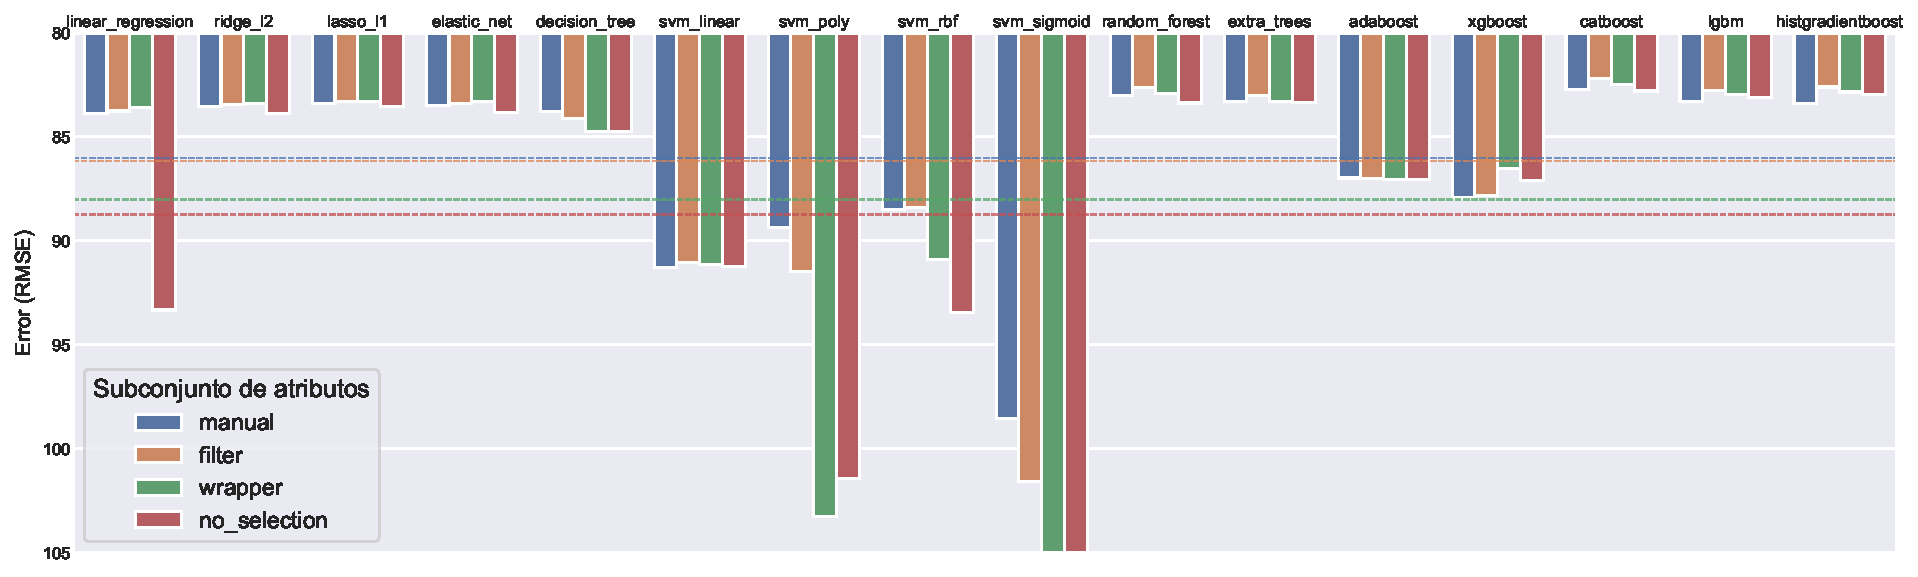
\includegraphics[width=1.1\linewidth]{figs/chapter5/training/error}}
	\captionsetup{belowskip=-15pt, justification=centering}
	\caption{Error promedio durante el entrenamiento para cada modelo y subconjunto de atributos (acotado en un error máximo de 105)}
	\label{fig:ch5trainerror}
\end{figure}

\subsubsection{Tiempo de entrenamiento}

\begin{figure}[h]
	\centering
	\makebox[\textwidth][c]{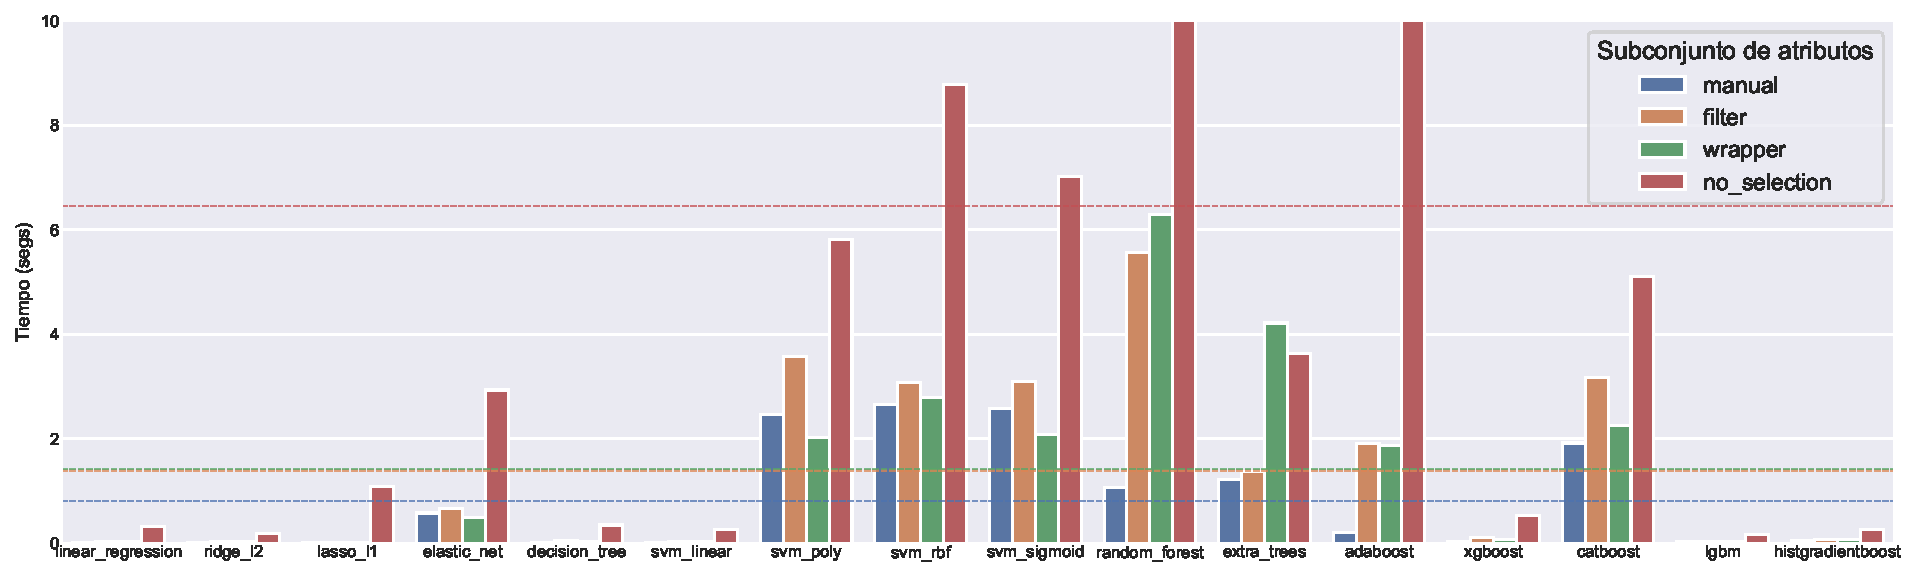
\includegraphics[width=1.1\linewidth]{figs/chapter5/training/time}}
	\captionsetup{belowskip=-15pt, justification=centering}
	\caption{Tiempo promedio de entrenamiento para cada modelo y subconjunto de atributos (acotado en 10 segundos)}
	\label{fig:ch5traintime}
\end{figure}

\subsection{Rendimiento de los modelos entrenados}

\subsubsection{Error de los modelos seleccionados}

\subsection{Rendimiento del modelo final}